\documentclass{article}

% Language setting
% Replace `english' with e.g. `spanish' to change the document language
\usepackage[english]{babel}

% Set page size and margins
% Replace `letterpaper' with`a4paper' for UK/EU standard size
\usepackage[letterpaper,top=2cm,bottom=2cm,left=3cm,right=3cm,marginparwidth=1.75cm]{geometry}

% Useful packages
\usepackage{amsmath}
\usepackage{graphicx}
\usepackage[colorlinks=true, allcolors=blue]{hyperref}

\title{Combinatorical analysis of burst failures for large-scale cluster}
\author{Meng Wang}

\begin{document}
\maketitle

\section{Setup}
We consider a storage system of N drives such that $N = X \cdot Y \cdot Z$, where there are $X$ racks in the system, each rack contains $Y$ enclosures, and each enclosure contains $Z$ drives.

Let $M = Y \cdot Z$, so $M$ denotes the number of drives per rack.

In particular, we are considering ORNL Alpine system, which is composed of 39 racks. 38 racks have 8 enclosures each, and 1 rack has 4 enclosures. Each enclosure has 106 drives.

For simplicity, we assume the system contains 40 racks. Each rack contains 8 enclosures. Each enclosure contains 100 drives.

\section{Total instances with fixed number of affected racks}

Consider $f$ failures happen in $r$ racks.

We first choose $r$ racks from all the $X$ racks, which has $C_{X}^{r}$ combinations.

Given $r$ racks $1,2,...,r$, denote $T(f,r)$ as the total number of instances for $f$ failures to happen in $r$ racks, such that each rack has at least one failure.

Consider the $r$-th rack. If it has $i$ failures, then the rest $r-1$ racks must have $(f-i)$ failures in total with each rack having at least one failure.

Therefore, we have the following recurrence relation:

\begin{eqnarray}
\begin{aligned}
  T(f,r)
  &= \sum_{\substack{1 \leq i \leq f \\ i \leq M}} C_M^i \cdot T(f-i, r-1)
\end{aligned}
\label{eq:total:rec}
\end{eqnarray}

The base case is 

\begin{eqnarray}
  T(f,1) =
    \begin{cases}
      C_M^f& \text{if $1 \leq f \leq M$}\\
      0 & \text{otherwise}
    \end{cases}       
\label{eq:total:base}
\end{eqnarray}

Therefore, we can compute $T(f,r)$ using dynamic programming, with time complexity $O(f \cdot r)$, and memory complexity $O(f \cdot r)$. An implementation can be found at: \url{https://github.com/ucare-uchicago/mlec-sim/blob/main/src/theory/policies/total.py}

The total number of instances is:
\begin{eqnarray}
  C_{X}^{r} \cdot T(f,r)
\label{eq:total:final}
\end{eqnarray}




\section{Survival instances under local clustered (RAID)}\label{sec-raid}

Consider $k_l+p_l$ local-only RAID SLEC. For easier deployment we assume $n_l=k_l+p_l$ is divisible by Z.

$n_l$ drives in the same enclosure compose a RAID disk group. Therefore a rack contains $g = M/n_l$ RAID groups.

\subsection{Survival counting in a single RAID group}

Denote $\Gamma(f, g)$ as the number of instances for one single rack to survive $f$ failures in a rack containing $g$ $k_l+p_l$ RAID groups.

For $\Gamma(f, g)$, we have the following recurrence relation (which is derived by considering what will happen if $g$-th group contains $i$ failures):

\begin{eqnarray}
\begin{aligned}
  \Gamma(f, g) &= \sum_{\substack{0 \leq i \leq p_l \\ a\leq f}} \Gamma(f-i, g-1) \cdot C_{n_l}^i
\end{aligned}
\label{eq:raid:1}
\end{eqnarray}

The base case is 

\begin{eqnarray}
  \Gamma(f, 1) =
    \begin{cases}
      C_{n_l}^f& \text{if $0 \leq f \leq n_l$}\\
      0 & \text{otherwise}
    \end{cases}       
\label{eq:raid:2}
\end{eqnarray}

We can then compute $\Gamma(f_i, g_l)$ based on recurrence relation \ref{eq:raid:1} and dynamic programming, with $O(f \cdot g)$ time complexity and $O(f \cdot g)$ memory complexity.


\subsection{Survival counting in entire system}

Given $r$ racks $1,2,...,r$, denote $S(f,r)$ as the total number of instances for $k_l+p_l$ local-only RAID to survive $f$ failures to in $r$ racks, such that each rack has at least one failure.

For $S(f,r)$, we have the following recurrence relation (which is derived by considering what will happen if $r$-th rack contains $i$ failures):

\begin{eqnarray}
\begin{aligned}
  S(f,r)
  &= \sum_{\substack{1 \leq i \leq f \\ i \leq M}} \Gamma(i,g) \cdot S(f-i, r-1)
\end{aligned}
\label{eq:raid:3}
\end{eqnarray}

The base case is 

\begin{eqnarray}
  S(f,1) =
    \begin{cases}
      \Gamma(f,g)& \text{if $1 \leq f \leq M$}\\
      0 & \text{otherwise}
    \end{cases}       
\label{eq:raid:4}
\end{eqnarray}

Since we have already computed $\Gamma(f,g)$, we can further compute $S(f,r)$ based on recurrence relation \ref{eq:raid:3} and dynamic programming. The total time complexity $O(f \cdot (g+r)$, and total memory complexity and $O(f \cdot (g+r)$.

Here is an example implementation: \url{https://github.com/ucare-uchicago/mlec-sim/blob/main/src/theory/policies/raid.py}

Therefore, the total number of survival instances in the whole system is:

\begin{eqnarray}
C_{X}^{r} \cdot S(f,r)
\label{eq:raid:5}
\end{eqnarray}

Therefore, the probability of data loss under $f$ failures on $r$ racks for RAID is:

\begin{eqnarray}
\begin{aligned}
\text{RAID data loss} = \frac{C_{X}^{r} \cdot S(f,r)} 
{C_{X}^{r} \cdot T(f,r)}
= \frac{ S(f,r)} { T(f,r)}
\end{aligned}
\label{eq:raid:6}
\end{eqnarray}



\section{Survival instances under local declustered parity}

It's similar to local clustered erasure in Section \ref{sec-raid}, but now the size of the disk group is usually larger than $n_l$. 

Suppose the size of the disk group is $D$, usually $n_l \leq D \leq Z$, where $Z$ is the size of the enclosure.

If any disk group has more than $p_l$ disk failures, then there is data loss.

So this time a rack contains $g = M/D$ disk groups.

We can then compute the data loss in the same way that we did for RAID. Therefore, the probability of data loss under $f$ failures on $r$ racks for local-only Declustered erasure is:

\begin{eqnarray}
\begin{aligned}
\text{Declustered data loss} = \frac{C_{X}^{r} \cdot S(f,r)} 
{C_{X}^{r} \cdot T(f,r)}
= \frac{ S(f,r)} { T(f,r)}
\end{aligned}
\label{eq:dp:1}
\end{eqnarray}




\section{Survival instances under network clustered erasure}

Consider $n_n=k_n+p_n$ network-only clustered erasure.

We first divide all the racks into $\alpha = X / n_n$ rack groups, each rack group with $n_n=k_n+p_n$ racks.

In each rack group, we further divide the disks into disk groups. Each disk group contains $n_n=k_n+p_n$ disks spread on $n_n$ racks, with each disk on a different rack.

\begin{center}
    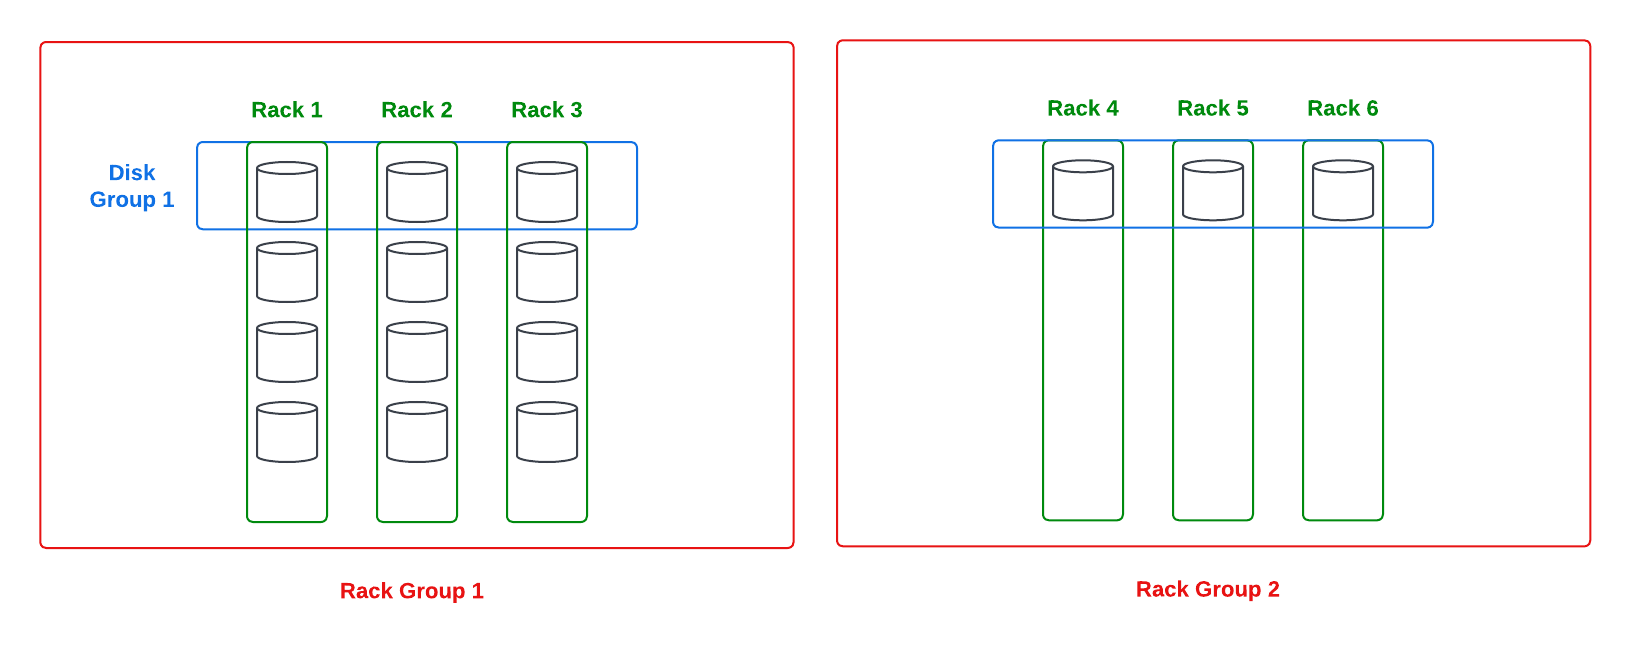
\includegraphics[width=0.9\textwidth]{netraid_layout.png}
\end{center}

\subsection{Survival counting in a single rack group}

Denote $\Gamma(f,r,m)$ as the number of instances for one rack group to survive $f$ failures in $r$ racks in this rack group, with each rack contains $m$ disks.

Thus there are $m$ disk groups in the rack group: $1,2,..., m$. Suppose the $m$-th disk group has $i$ failures spread in $i$ racks. Then disk group $1,2,...,m-1$ should have $f-i$ failures in total. Suppose these $f-i$ failures spread in $j$ racks. Then the $i$ racks affected by disk group $m$ and the $j$ racks affected by disk groups $1...m-1$ must overlap on $i+j-r$ racks. And there are $r-j$ racks which are affected by disk group $m$ only.

If we consider of the possible values of $i$ and $j$, we can derive the following recurrence relation for $\Gamma(f,r,m)$ :

\begin{eqnarray}
\begin{aligned}
  \Gamma(f,r,m) &= \sum_{\substack{0 \leq i \leq p_n \\ i\leq r}} 
                \sum_{\substack{0 \leq j \leq r \\ r-i \leq j}}
                C_{j}^{i+j-r} \cdot C_{n_n-j}^{r-j} \cdot \Gamma(f-i, j, m-1) 
\end{aligned}
\label{eq:netraid:1}
\end{eqnarray}

The base case is 

\begin{eqnarray}
  \Gamma(f,1,m) =
    \begin{cases}
      C_{m}^f \cdot C_{n_n}^1 & \text{if $0 \leq f \leq m$}\\
      0 & \text{otherwise}
    \end{cases}       
\label{eq:netraid:2}
\end{eqnarray}

We can then compute $\Gamma(f,r,M)$ based on recurrence relation \ref{eq:netraid:1} and dynamic programming, with $O(f \cdot r \cdot M)$ time complexity and $O(f \cdot r \cdot M)$ memory complexity.


\subsection{Survival counting in the entire system}

Given $\alpha$ rack groups $1,2,...,\alpha$, denote $S(f,r, \alpha)$ as the total number of instances for $n_n=k_n+p_n$ network-only RAID to survive $f$ failures in $r$ racks, such that each rack has at least one failure.

For $S(f,r,\alpha)$, we have the following recurrence relation (which is derived by considering what will happen if $\alpha$-th rack group contains $i$ failures affecting $j$ racks):

\begin{eqnarray}
\begin{aligned}
  S(f,r,\alpha)
  &= \sum_{\substack{0 \leq i \leq f \\ i \leq M*p_n}}
  \sum_{\substack{0 \leq j \leq r \\ j \leq i \\ j \leq n_n}}
  \Gamma(i,j,M) \cdot S(f-i, r-j, \alpha-1)
\end{aligned}
\label{eq:netraid:3}
\end{eqnarray}

The base case is 

\begin{eqnarray}
  S(f,r,1) =  \Gamma(f,r,M)
\label{eq:netraid:4}
\end{eqnarray}

Since we have already computed $\Gamma(f,r,m)$, we can further compute $S(f,r,\alpha)$ based on recurrence relation \ref{eq:netraid:3} and dynamic programming. The total time complexity $O(f \cdot r \cdot \alpha)$, and total memory complexity and $O(f \cdot r \cdot \alpha)$.

An example implementation can be found at: \url{https://github.com/ucare-uchicago/mlec-sim/blob/main/src/theory/policies/netraid.py}






\section{Survival instances under network declustered erasure}

This is easy.

Consider $n_n=k_n+p_n$ network-only declustered erasure.

There is data loss whenever there are more than $p_n$ affected racks.

Therefore:

\begin{eqnarray}
  \text{Net-declus Data loss} =
    \begin{cases}
      1 & \text{if $r > p_n$}\\
      0 & \text{otherwise}
    \end{cases}       
\label{eq:net_dp:1}
\end{eqnarray}

where $r$ is the number of affected racks.






\section{Survival instances under MLEC clustered}\label{sec-mlec}

Consider $(k_n+p_n)/(k_l+p_l)$ clustered MLEC.
We first divide all the racks into $\alpha = X / n_n$ rack groups, each rack group with $n_n=k_n+p_n$ racks.

In each rack group, we further divide the disks into mlec groups. Each mlec group contains $n_n=k_n+p_n$ disks on a different rack, thus $n_n \cdot n_l$ disks in total.

The following figure shows $(2+1)/(2+1)$ clustered MLEC layout among 6 racks.

\begin{center}
    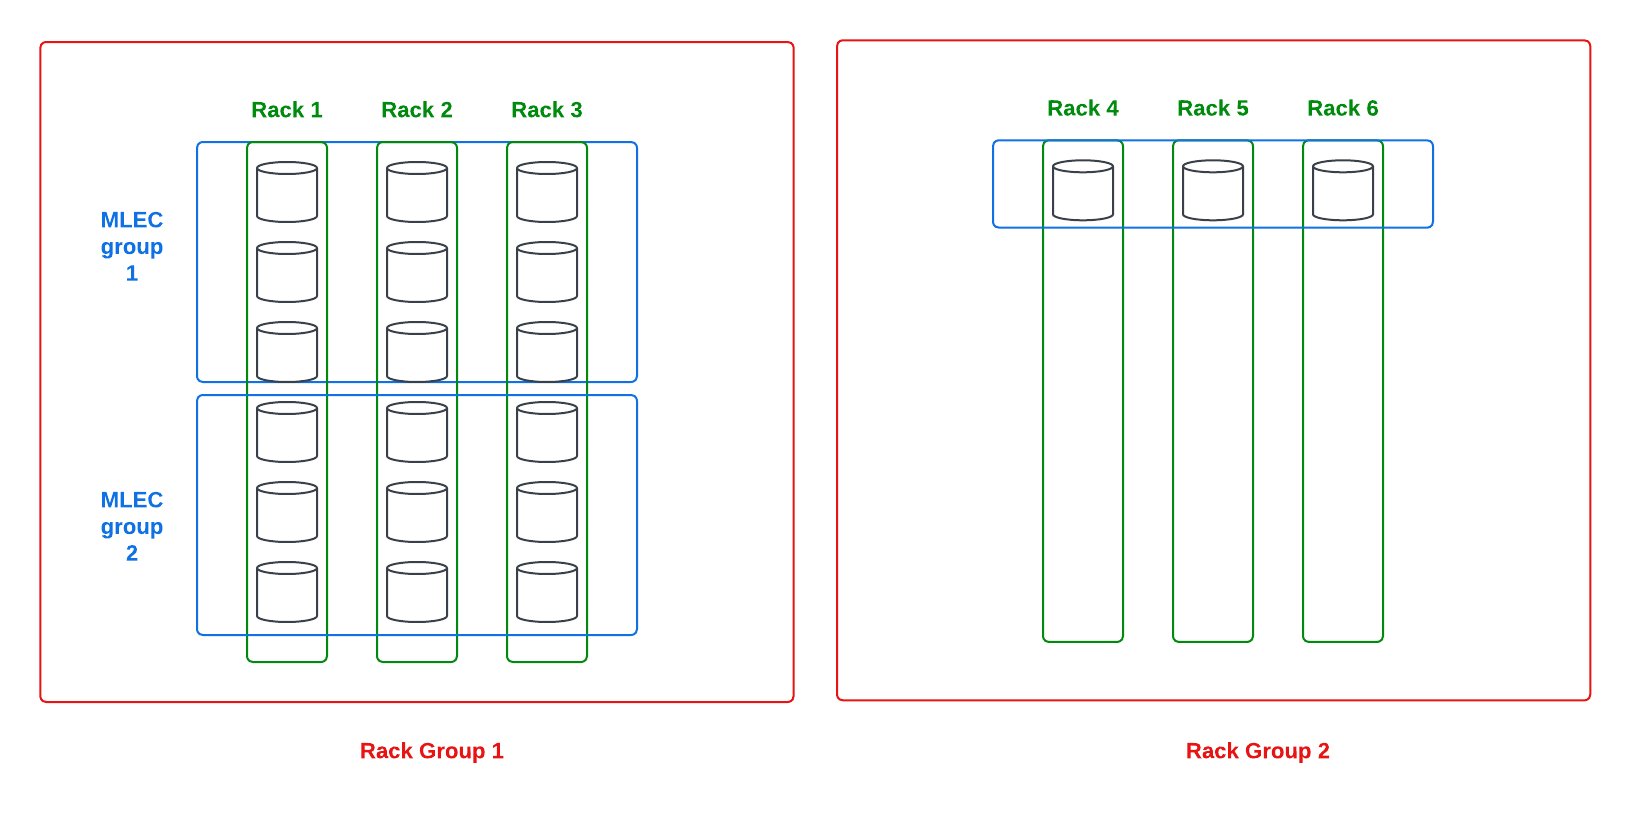
\includegraphics[width=0.9\textwidth]{mlec_layout.png}
\end{center}


\subsection{Count survivals in a single mlec group}

Consider a disk group spread among $a$ racks, with each rack containing $n_l=k_l+p_l$ disks. Each rack can survive at most $p_l$ disk failures.
The whole disk group can survive at most $p_n$ rack failures. 

Denote $\Theta(a,p_n,f,r)$ as the number of instances for such a disk group to survive $f$ failures in $r$ racks in this rack group.

Assume the $a$-th rack contains $i$ disk failures. 
If we consider of the possible values of $i$, we can derive the following recurrence relation for $\Theta(a,p_n,f,r)$ :

\begin{eqnarray}
\begin{aligned}
  \Theta(a,p_n,f,r) &= \sum_{\substack{0 \leq i \leq n_l \\ i\leq f}} 
                \Delta(a,p_n,f,r, i)
\end{aligned}
\label{eq:mlec:1}
\end{eqnarray}

where:

\begin{eqnarray}
  \Delta(a,p_n,f,r, i) =
    \begin{cases}
      \Theta(a-1,p_n,f,r) & \text{if $i = 0$}\\
      C_{n_l}^{i} \cdot \Theta(a-1,p_n,f-i,r-1) & \text{if $i \leq p_l$} \\ 
      C_{n_l}^{i} \cdot \Theta(a-1,p_n-1,f-i,r-1) & \text{if $i > p_l$}
    \end{cases}       
\label{eq:mlec:2}
\end{eqnarray}



The base case is 

\begin{eqnarray}
  \Theta(a,p_n,f,0) =
    \begin{cases}
      1 & \text{if $f=0$}\\
      0 & \text{otherwise}
    \end{cases}       
\label{eq:mlec:3}
\end{eqnarray}

Then the survival counting for a mlec group is $\Theta(n_n,p_n,f,r)$.

With dynamic programming, the time complexity and space complexity to compute $\Theta(a,p_n,f,r)$ are both $O(n_n \cdot p_n \cdot f \cdot r)$

\subsection{Count survivals in a single rack group}






Denote $\Gamma(f,r,m)$ as the number of instances for one rack group to survive $f$ failures in $r$ racks in this rack group.

The rack group contains $m = M / n_l$ mlec groups. Suppose the $m$-th rack group has $i$ failures spread in $j$ racks. Then mlec group $1,2,...,m-1$ should have $f-i$ failures in total. Suppose these $f-i$ failures spread in $h$ racks. Then the $j$ racks affected by disk group $m$ and the $h$ racks affected by disk groups $1...m-1$ must overlap on $j+h-r$ racks. And there are $r-h$ racks which are affected by disk group $m$ only.

If we consider of the possible values of $i$,$j$, and $h$, we can derive the following recurrence relation for $\Gamma(f,r,m)$ :

\begin{eqnarray}
\begin{aligned}
  \Gamma(f,r,m) &= \sum_{\substack{0 \leq i \leq f}} 
                \sum_{\substack{0 \leq j \leq r}}
                \sum_{\substack{0 \leq h \leq r \\ r-j \leq h}}
                C_{j}^{j+h-r} \cdot C_{n_n-h}^{r-h} \cdot \Theta(j,p_n,i,j)
                \cdot \Gamma(f-i, h, m-1) 
\end{aligned}
\label{eq:mlec:4}
\end{eqnarray}

The base case is 

\begin{eqnarray}
  \Gamma(0,h,m) =
    \begin{cases}
      1 & \text{if $h=0$}\\
      0 & \text{otherwise}
    \end{cases}       
\label{eq:mlec:5}
\end{eqnarray}

With dynamic programming, the time complexity and space complexity to compute $\Gamma(f,r,m)$ are both $O(f \cdot r \cdot m)$

\subsection{Survival counting in the entire system}

Given $\alpha$ rack groups $1,2,...,\alpha$, denote $S(f,r, \alpha)$ as the total number of survivals under $f$ failures in $r$ affected racks.

For $S(f,r,\alpha)$, we have the following recurrence relation (which is derived by considering what will happen if $\alpha$-th rack group contains $i$ failures affecting $j$ racks):

\begin{eqnarray}
\begin{aligned}
  S(f,r,\alpha)
  &= \sum_{\substack{0 \leq i \leq f \\ i \leq M*n_n}}
  \sum_{\substack{0 \leq j \leq r \\ j \leq i \\ j \leq n_n}}
  \Gamma(i,j,M/n_l) \cdot S(f-i, r-j, \alpha-1)
\end{aligned}
\label{eq:mlec:6}
\end{eqnarray}

The base case is 

\begin{eqnarray}
  S(f,r,1) =  \Gamma(f,r,M/n_l)
\label{eq:mlec:7}
\end{eqnarray}

Since we have already computed $\Gamma(f,r,m)$, we can further compute $S(f,r,\alpha)$ based on recurrence relation \ref{eq:mlec:6} and dynamic programming. The total time complexity $O(f \cdot r \cdot \alpha)$, and total memory complexity and $O(f \cdot r \cdot \alpha)$.

The aggregate time complexity is $O(f \cdot r \cdot (n_n p_n + \frac{M}{n_l} + \frac{X}{n_n}))$

An example implementation can be found at: \url{https://github.com/ucare-uchicago/mlec-sim/blob/main/src/theory/policies/mlec.py}







\section{Survival instances under MLEC Declustered}

This is very similar to MLEC clustered in section \ref{sec-mlec}. The only difference is that now an mlec group contains $D$ disks per rack, where $D$ is the local disk group size in local declustered parity.

Therefore, equation \ref{eq:mlec:2} should be changed to:

\begin{eqnarray}
  \Delta(a,p_n,f,r, i) =
    \begin{cases}
      \Theta(a-1,p_n,f,r) & \text{if $i = 0$}\\
      C_{D}^{i} \cdot \Theta(a-1,p_n,f-i,r-1) & \text{if $i \leq p_l$} \\ 
      C_{D}^{i} \cdot \Theta(a-1,p_n-1,f-i,r-1) & \text{if $i > p_l$}
    \end{cases}       
\label{eq:mlec_dp:1}
\end{eqnarray}

The survival counting for a rack group now equals: $\Gamma(f,r,\frac{M}{D})$

The recurrence of surviving counting for the entire system now equals:

\begin{eqnarray}
\begin{aligned}
  S(f,r,\alpha)
  &= \sum_{\substack{0 \leq i \leq f \\ i \leq M*n_n}}
  \sum_{\substack{0 \leq j \leq r \\ j \leq i \\ j \leq n_n}}
  \Gamma(i,j,M/D) \cdot S(f-i, r-j, \alpha-1)
\end{aligned}
\label{eq:mlec_dp:2}
\end{eqnarray}

with base case $S(f,r,1) =  \Gamma(f,r,M/D)$.

The aggregate time complexity is $O(f \cdot r \cdot (n_n p_n + \frac{M}{D} + \frac{X}{n_n}))$

An example implementation can be found at: \url{https://github.com/ucare-uchicago/mlec-sim/blob/main/src/theory/policies/mlec_dp.py}


\end{document}